\vspace{-12pt}
\section{Evaluation of Policies Learned by the Language Model}
\label{sec:eval_policy}
We ask the following research questions to evaluate the learned policies:


\textbf{RQ1} (Effect of behaviour): How much does the change in behaviour alone contribute to the success of the attack v/s the change in internal activations? 

\textbf{RQ2} (Generalisation): Does the learned policy highly depend on the probe architecture? Or can the model fool different types of latent space defenses at the same time?

\begin{result}
{
\textbf{   \em Key Takeaways:}
}
\begin{itemize}
    \item The black-box behavior is responsible for most of the evasion observed. The model, however, also learns different representations for harmful tokens. 
    \item RL-Obfuscation on one type of static probe generalises to other types of static probes as well, unless using maxpool probes or attention-based probes. 
\end{itemize}
\end{result}
% \vspace{-12pt}
% \subsection{Results}
\begin{figure}[t]
    \centering
    \begin{subfigure}[b]{0.4\textwidth}
        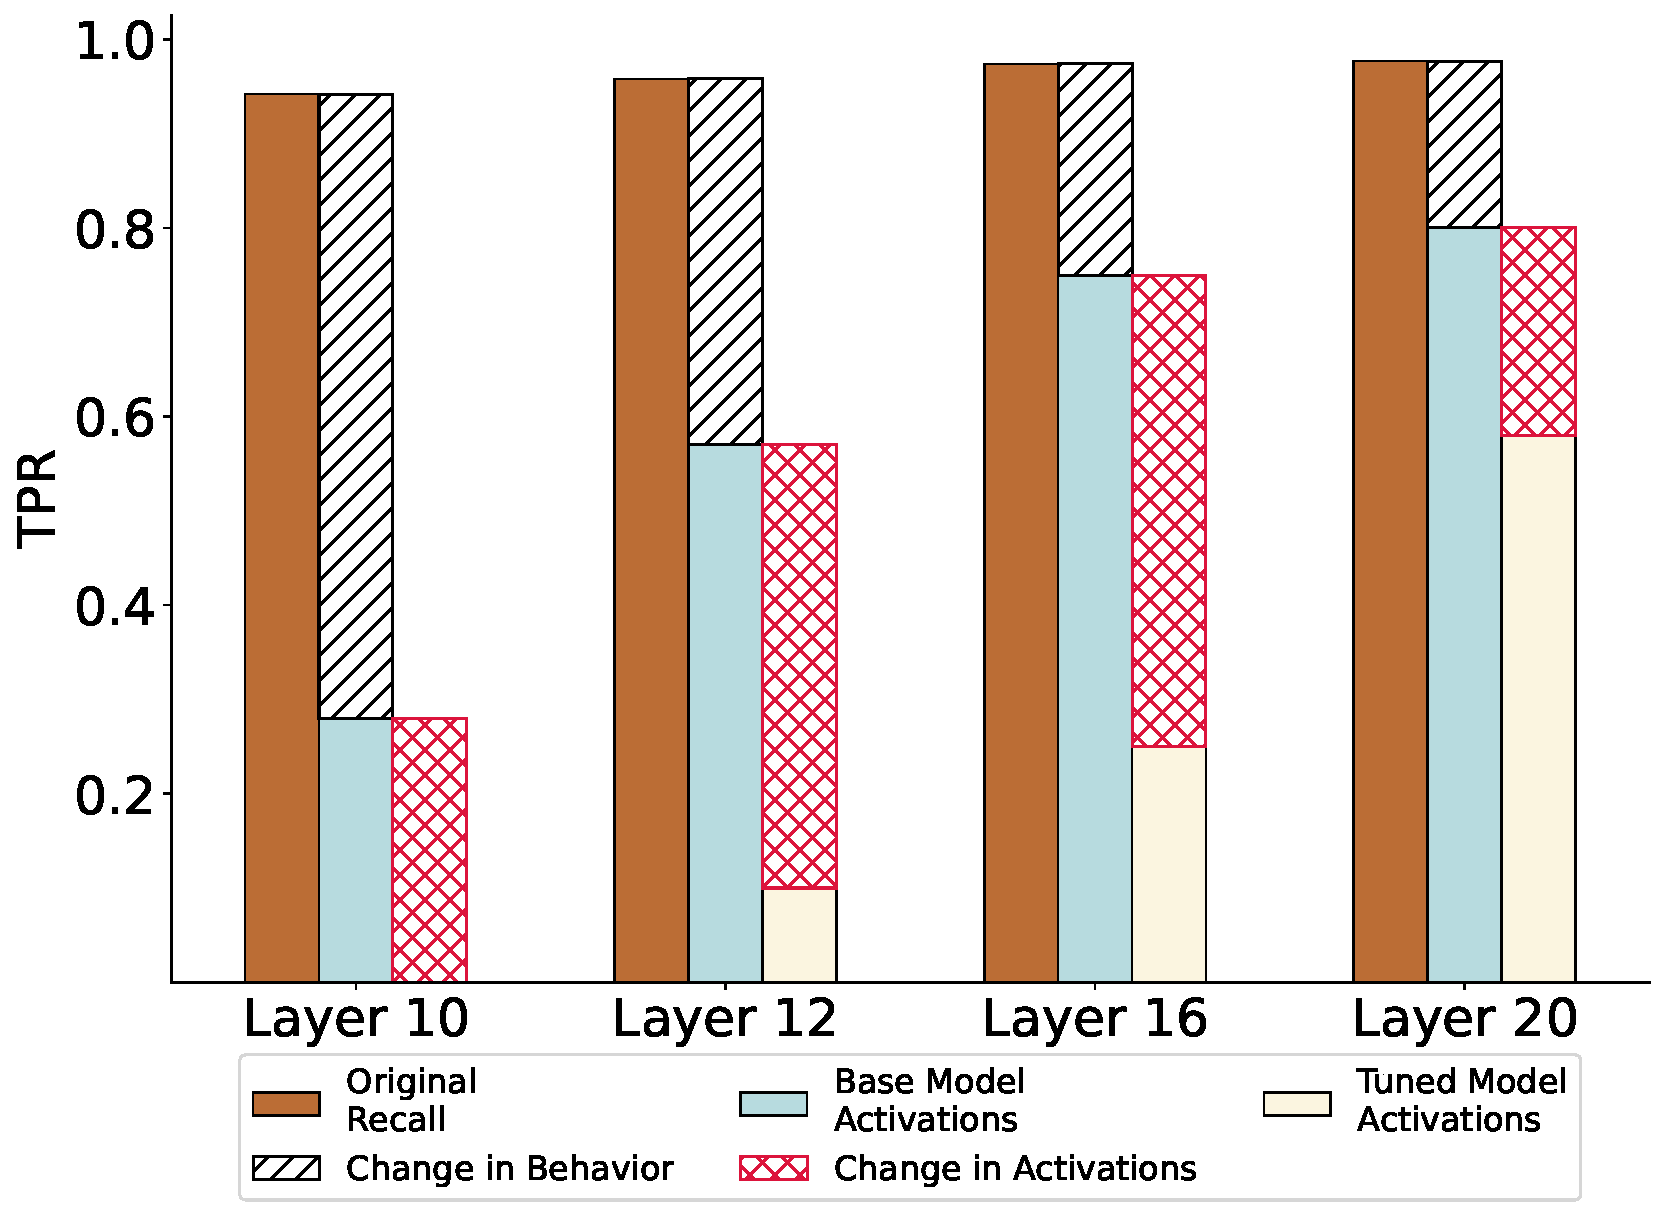
\includegraphics[width=\textwidth]{figures/behavior_vs_acts.pdf}
        \caption{}
        \label{fig:behavior_vs_acts}
    \end{subfigure}
    \hfill
    \begin{subfigure}[b]{0.55\textwidth}
        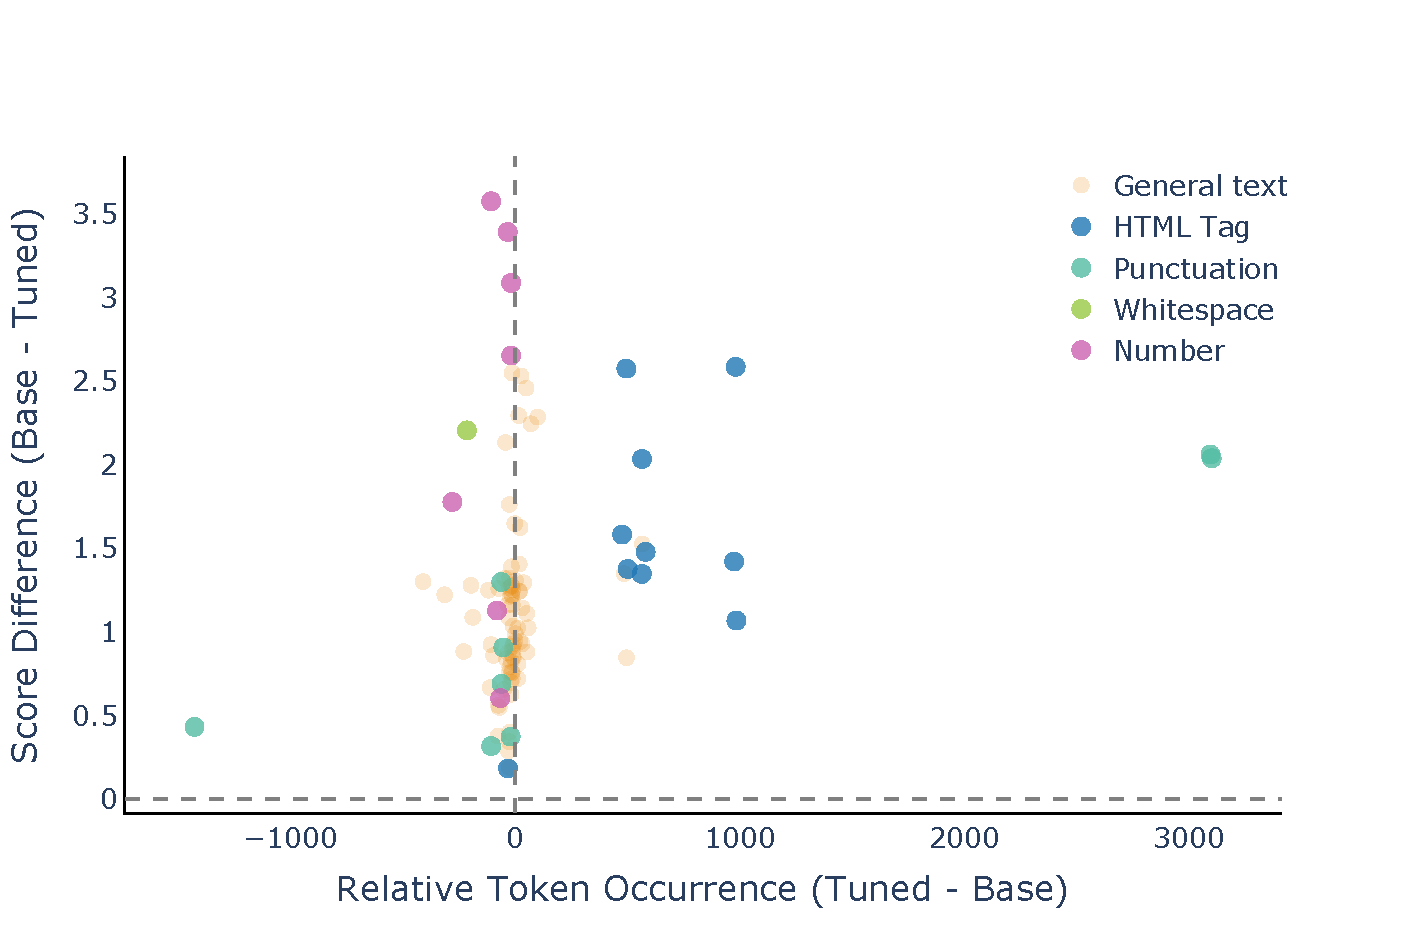
\includegraphics[width=\textwidth]{figures/token_score_vs_occurrence.pdf}
        \caption{}
        \label{fig:per_token_diff}
    \end{subfigure}
    % \caption{Comparison between behavioral changes and activation manipulation in probe evasion. The left plot shows that RL training achieves greater probe accuracy drops than teacher forcing alone, indicating the model learns to manipulate its activations beyond just changing behavior. The right plot analyzes how specific tokens' activations differ between the two approaches while maintaining similar output behavior.\todo{Improve caption, make plots pdfs}}

    \caption{\textbf{(a)} Whitebox Monitor recall at $0.5\%$ FPR for various layers. The brown bars show the original recall of the monitor on the base model. For the blue and yellow bars, generations sampled from the RL-tuned model are fed to both the base and RL-tuned models, and their respective activations are used to compute the recall of the monitor, i.e., $\modelLayerScore{\rlPolicy}{\baseModel}{L}$ and $\modelLayerScore{\rlPolicy}{\rlPolicy}{L}$, respectively in \Cref{eq:model_layer_score}.  
    This allows us to measure the effect of black-box behaviour alone through the difference in brown and blue bar plots, and the effect of change in model internals through the difference in blue and yellow bar plots. 
    % This reveals that changes in activations contribute significantly towards evading probes and not just behavioral changes.
    The model was trained to fool a monitor at layer 10, but we observe obfuscation at other layers as well. 
    \textbf{(b)} Per-token probe logit difference between the two models at layer 10 v/s the relative occurrence of tokens in base and tuned model generations. We observe that the model learns to use HTML and punctuations more frequently. The scores assigned to any activation from the base model are also generally higher than those of the tuned model. % \vspace{-24pt}
}
    % \label{fig:behavior_vs_acts}
\end{figure}

\paragraph{RQ1. (Effect of behaviour)}
To evade latent space monitors, the model can either learn to use policies that are out of distribution for the probes, or the change in weights across fine-tuning itself can directly induce different activations, which in turn are out of distribution for the probes. In \Cref{fig:behavior_vs_acts}, we isolate the effect of change in behaviour and change in activations during RL-Obfuscation. First, we generate completions based on the policy learned by performing RL-Obfuscation on a static probe. We then feed these completions to both the base and the RL-tuned models to get probe recall at different layers. Formally, this can be denoted as: 
\begin{align}
    \modelLayerScore{\rlPolicy}{M}{L} = \expectation{(\modelCompletion\sim \rlPolicy|x), (x\sim \text{Unsafe})}\left[\layerMonitor{L}(\modelActivations{M}{x}{y}{L})\right], \quad M\in \{ \baseModel,  \rlPolicy\}
    \label{eq:model_layer_score}
\end{align}

where $\rlPolicy$ and $\baseModel$ are the RL-tuned model and the base model respectively, $L$ is a particular layer in the model and $\layerMonitor{L}(.)$ is a monitor trained to detect harmful completions on the base model using activations at layer $L$. The model was trained using \setupStatic \space from \Cref{sec:problem_setup} until the model completely evades the monitor at $0.5\%$ FPR. 
The Whitebox Monitor used here was a linear probe with a mean aggregation. All probes used to compute recall were trained on the base model. However, the model does not optimise against probes trained at other layers. 

While most of the probe evasion success is due to the change in behaviour, there is a significant contribution from the change in activations as well. To test this difference even further, we train a linear probe on the base model, when token-forced with the tuned model's generations on harmful prompts in \Cref{fig:base_model_on_tuned_completions}. We see a similar difference here as well.

\Cref{fig:per_token_diff} shows a more fine-grained picture of the changes in behaviour and activations. We use the same experimental setup as described above and plot the mean unnormalised probe logit difference at layer 10, when both models are fed completions from the tuned model ($\modelCompletion \sim \rlPolicy$). We categorise each token using simple regular expressions.
% \newpage
We observe the following two changes:
\begin{enumerate}
    \item Change in overall activations:
    
    Activations on the same policy are scored generally higher with respect to the tuned model. This is a global phenomenon and occurs throughout the generations. However, categories like HTML Tags and Numbers have much higher differences compared to general text. \Cref{fig:main} additionally shows this change in activations along the top two principal components explaining activations of a dataset containing 100 benign generations from $\rlPolicy$ and 100 unsafe generations from $\baseModel$ and $\rlPolicy$ each.
    
    \item Learning a different black-box behavior that evades probes:

    The tuned model learns to use certain categories of text, like HTML tags and punctuations, with a relatively high frequency and a low probe score. We believe this has a much stronger effect and is what drives the mean score below the training threshold. Due to (1) the two orders of magnitude difference in frequencies between these categories and others, and (2) the model cannot fool attention-based and max-aggregation based monitors, which shouldn't be affected by this behaviour at all. Other types of black-box behaviour learned after RL-Obfuscation are displayed in \Cref{fig:main}.
\end{enumerate}
% \vspace{-4pt}
These two factors—and the magnitude of their effects—explain the trend observed in \Cref{fig:per_token_diff}, where the change in policy contributes to approximately $70\%$ of the drop in recall.  

\begin{figure}[t]
    \centering
    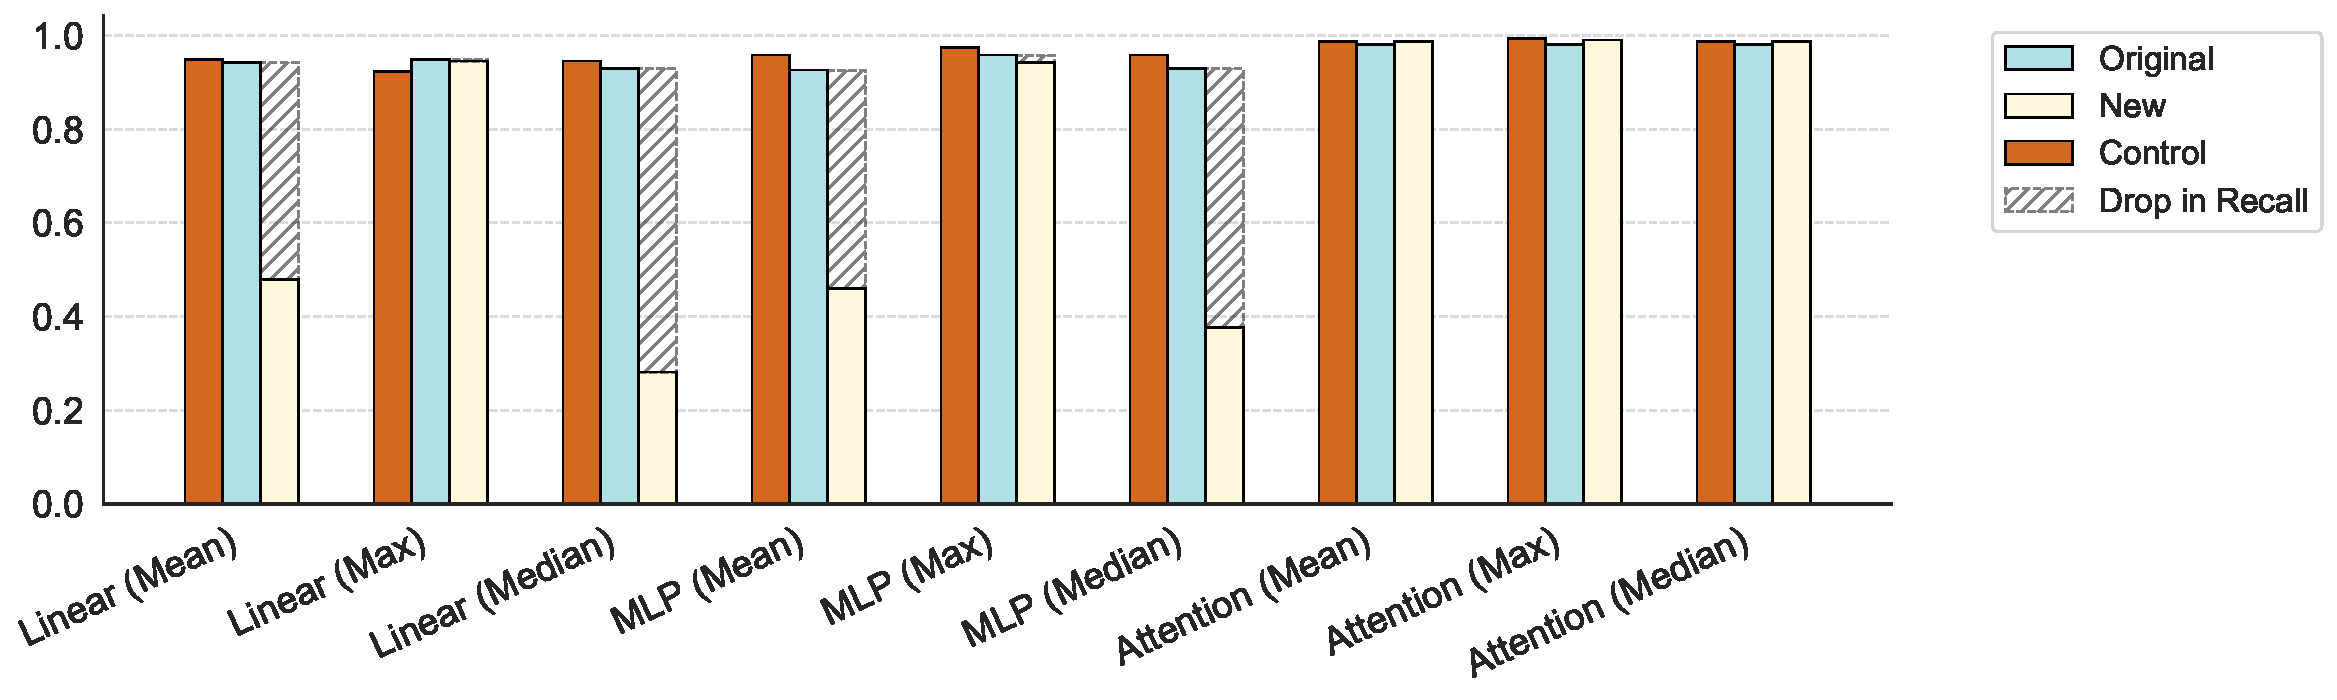
\includegraphics[width=0.9\linewidth]{figures/rl_obfuscation_other_probes.pdf}
    \caption{
    Effect of RL-Obfuscation on other probes: Accuracy of probes to detect harmful generations (recall) generated by three models: helpful-only base model (blue), a model trained to evade linear probes (yellow), and a control model trained to only maximise the StrongReject grader (brown). \vspace{-12pt}
    }
    \label{fig:generalization}
\end{figure}
% \vspace{-4pt}
\paragraph{RQ2. (Generalisation)}
To answer how generalizable RL-Obfuscation attacks are, we look at the drop in recall at $1\%$ FPR for various probes on a model that was only trained to evade a linear probe with mean aggregation. The model was trained using \setupStatic \space from \Cref{sec:problem_setup}. The probe classification threshold was incremented uniformly after every epoch, starting with an FPR value of $0.3\%$, for 3 epochs. As in \Cref{sec:compare_probes}, the MLP (max aggregation) monitor was trained with maxpooling. 

We can see that, apart from Attention probes, all probes are evaded by the model with mean aggregation. We also see that any probe with max aggregation cannot be evaded. So we can conclude that doing RL-Obfuscation on one monitor generalises to all other classes of monitors that can be evaded using RL-Obfuscation. 
